\documentclass[11pt, a4paper]{report}
\usepackage{etoolbox}
\makeatletter
\patchcmd{\chapter}{\if@openright\cleardoublepage\else\clearpage\fi}{}{}{}
\makeatother
\usepackage[margin=1in]{geometry}
\usepackage[utf8]{inputenc} % Umožňuje psaní českých znaků
\usepackage[czech]{babel}   % Česká lokalizace pro babel
\usepackage{titlesec}
\usepackage{pdfpages}
\usepackage{tabularx}
\usepackage{xcolor}
\usepackage{hyperref}  % or \usepackage{url}


\titleformat{\chapter}
  {\normalfont\LARGE\bfseries}{\thechapter}{1em}{}
\titlespacing*{\chapter}{0pt}{3.5ex plus 1ex minus .2ex}{2.3ex plus .2ex}
\begin{document}
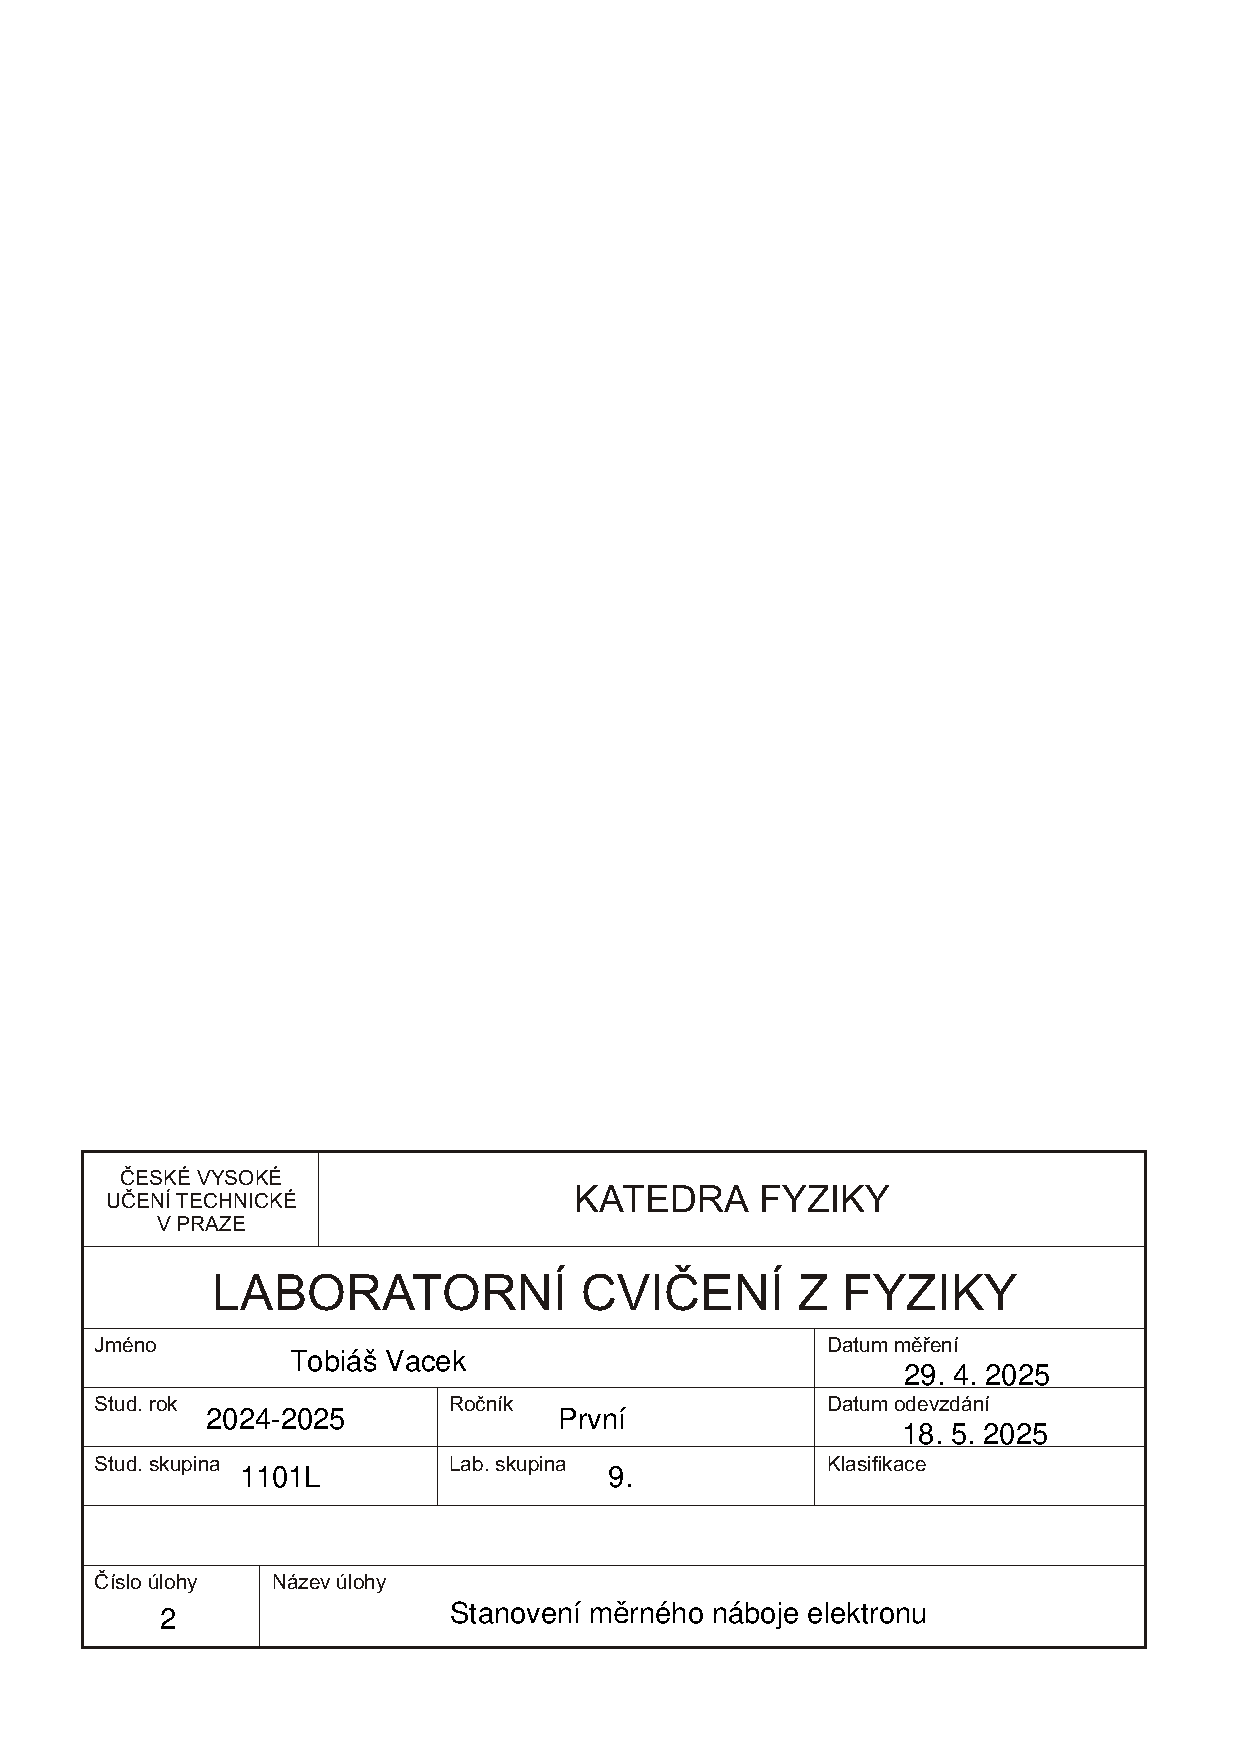
\includepdf{stamp.pdf}
\chapter{Úkol měření}
\begin{enumerate}
	\item Ze zakřivení drah elektronů pohybujících se v magnetickém poli stanovte \emph{měrný náboj elektronu.}
\end{enumerate}

\chapter{Použité přístroje}

\begin{center}
	\begin{tabularx}{\textwidth}{|>{\centering\arraybackslash}X
		|>{\centering\arraybackslash}X
		|>{\centering\arraybackslash}X
		|>{\centering\arraybackslash}X
		|>{\centering\arraybackslash}X|}
		\hline
		\textbf{Počet} & \textbf{Pomůcka} & \textbf{číslo} & \textbf{Přesnost}        & \textbf{Rozsah} \\
		\hline
		1              & ampérmetr        & MY-65          & \pm 2\,\% (\pm 5 digitů) & 10\,A           \\
		\hline
		1              & voltmetr         & MY-64          & \pm0,8\,\% (\pm2 digity) & 1000\,V         \\
		\hline
	\end{tabularx}
\end{center}

\chapter{Naměřené hodnoty a vypočtené hodnoty}
\begin{center}
	\renewcommand{\arraystretch}{1.5}
	\begin{table}[h]
		\centering
		%\renewcommand{\arraystretch}{1.5} % pro větší výšku řádků
		\begin{tabular}{|c|c|c|c|c|c|c|c|c|c|c|c|c|c|}
			\hline

			\textbf{Poloměr zakřivení } [cm]           & 2    & 2    & 2    & 2    & 3    & 3    & 3    & 3    \\
			\hline

			\textbf{Urychlovací napětí}  [V]           & 129  & 174  & 210  & 250  & 135  & 175  & 210  & 250  \\
			\hline
			\textbf{Proud cívkou} [A]                  & 2.66 & 3.33 & 3.69 & 3.99 & 1.64 & 2.16 & 2.38 & 2.60 \\
			\hline
			Magnetická indukce  [mT]                   & 1,84 & 2,31 & 2,55 & 2,76 & 1,14 & 1,50 & 1,65 & 1,80 \\
			\hline
			Měrný náboj $[10^{11}\;C \cdot kg^{-1} ]$  & 1.90 & 1.63 & 1.60 & 1.63 & 2.32 & 1.73 & 1.71 & 1.71 \\
			\hline
			\hline
			\textbf{Poloměr zakřivení} [cm]            & 4    & 4    & 4    & 4    & 5    & 5    & 5    & 5    \\
			\hline

			\textbf{Urychlovací napětí} [V]            & 150  & 190  & 220  & 250  & 150  & 190  & 220  & 250  \\
			\hline
			\textbf{Proud cívkou} [A]                  & 1.41 & 1.66 & 1.81 & 1.93 & 1.13 & 1.32 & 1.46 & 1.56 \\
			\hline
			Magnetická indukce [mT]                    & 0,98 & 1,15 & 1,25 & 1,34 & 0,78 & 0,91 & 1,01 & 1,08 \\
			\hline
			Měrný náboj $ [10^{11}\;C \cdot kg^{-1} ]$ & 1.96 & 1.79 & 1.75 & 1.75 & 1.96 & 1.81 & 1.72 & 1.71 \\
			\hline
		\end{tabular}
	\end{table}
\end{center}
\clearpage

\chapter{Výpočet}
\section{Měrný náboj}
Magnetickou indukci B jsme vypočetli podle vzorce:
\begin{center}
	\LARGE
	$B = \frac{8}{5\sqrt{5}}\frac{\mu_0NI}{a}$
\end{center}
kde $\mu_0 = 4\pi\cdot 10^{-7} N\cdot A^{-2}$ je magnetická konstanta, $N = 154$ je počet závitů cívky, $I$ je proud procházející cívkou
a $a = 0.2\, m$ je poloměr cívky.
\newline
\newline
S pomocí magnetické indukce jsme vypočetli měrný náboj elektronu $\frac{e}{m_e}$ podle vzorce:
\begin{center}
	\LARGE
	$ \frac{e}{m_e} = \frac{2U}{B^2 R^2_c}$
\end{center}
kde $U$ je urychlovací napětí, $B$ je magnetická indukce a $R_c$ je poloměr zakřivení dráhy elektronu.
\newline
\newline
Výpočet průměrné hodnoty měrného náboje a směrodatné odchylky:
\begin{center}
	\Large
	\[\overline{\;\frac{e}{m_e}\;} = \frac{\sum_{i=0}^{n}\frac{e}{m_e}_i}{n}= 1.7979\cdot 10^{11} C\cdot kg^{-1}\]
	\newline
	$ \sigma = \sqrt{\frac{\sum_{i=0}^{n}(\overline{x}-x_i)^2}{n(n-1)}} = 1.23\cdot 10^{10} C\cdot kg^{-1}$
\end{center}
pro zpřesnění výpočtu měrného náboje, byly z výpočtu odstraněny hodnoty, které se od průměru liší o více než je směrodatná odchylka.
\newline
\begin{figure}[h] % 'h' means place the figure approximately "here"
    \centering
    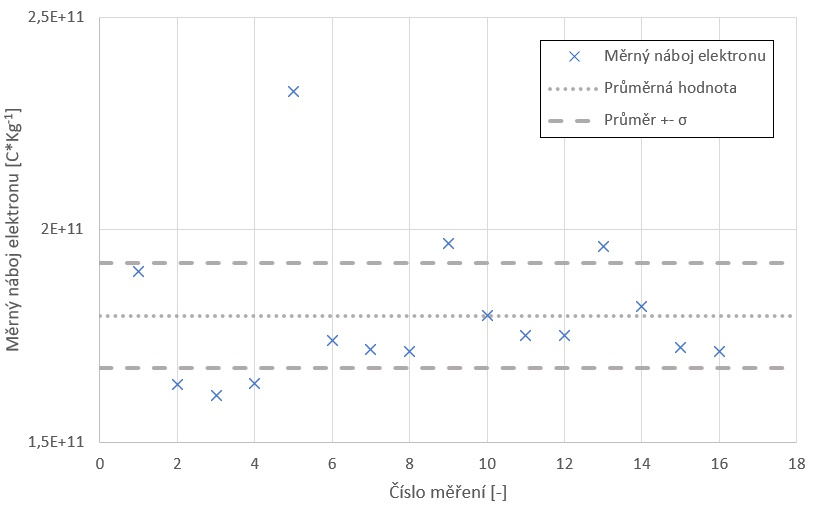
\includegraphics[scale = 0.55]{mer_naboj_graf.jpg}
    \caption{Graf měrného náboje elektronu s vyznačenou směrodatnou odchylkou}
    \label{fig:example_image} % optional label for referencing
\end{figure}
\clearpage
Po odstranění těchto hodnot se průměrná hodnota měrného náboje elektronu, změnila na:
\begin{center}
	\Large
	$\overline{\;\frac{e}{m_e}\;} = 1.7629\cdot 10^{11} C\cdot kg^{-1}$
\end{center}
\section{Nejistoty}
\subsection{Nejistota magnetické indukce}
\begin{center}
	\Large
	$u_b(I) = \frac{\textnormal{nejmenší dílek}}{\sqrt{12}}=\frac{0.01}{\sqrt{12}} = 0.003A$\\
	\vspace{0.2cm}
	$u_c(B) = \sqrt{(\frac{\partial B}{\partial I}\cdot u_b(I))^2}=0.69 mT$\\
\end{center}
\subsection{Nejistota měrného náboje}
\begin{center}
	\Large
	$u_b(U) = \frac{\textnormal{nejmenší dílek}}{\sqrt{12}}=\frac{1}{\sqrt{12}} = 0.28V$\\
	\vspace{0.5cm}
	\LARGE
	$u_c(\frac{e}{m_e})=\frac{\sum_{i=0}^{n}\sqrt{(\frac{\partial \frac{e}{m_e}}{\partial U_i}\cdot u_b(U))^2+(\frac{\partial \frac{e}{m_e}}{\partial B_i }\cdot u_c(B))^2}}{n}= 1.11\cdot 10^{9} C\cdot kg^{-1}$
\end{center}
\chapter{Závěr}
Ze zakřivení drah elektronů jsme určili, že měrný náboj elektronu je \mbox{$\frac{e}{m_e} = (1.76\pm0.01) \cdot 10^{11} C\cdot kg^{-1}$}.
Tato hodnota se od tabulkové hodnoty $\frac{e}{m_e} = 1.75\cdot 10^{11} C\cdot kg^{-1}$ liší o 0,2\%.

\chapter{Literatura}
\begin{enumerate}
	\item \url{https://physics.nist.gov/cgi-bin/cuu/Value?esme|search_for=electron+charge}
	\item \url{https://planck.fel.cvut.cz/praktikum/downloads/navody/mernab.pdf}
	\item \url{https://planck.fel.cvut.cz/praktikum/pristroje.php}
\end{enumerate}
\end{document}

